    \begin{frame}{\ft{Building Parsing Models}}
\section{Group 1: Building Parsing Models}

        \begin{annotatedFigure}{10pt}{0pt}{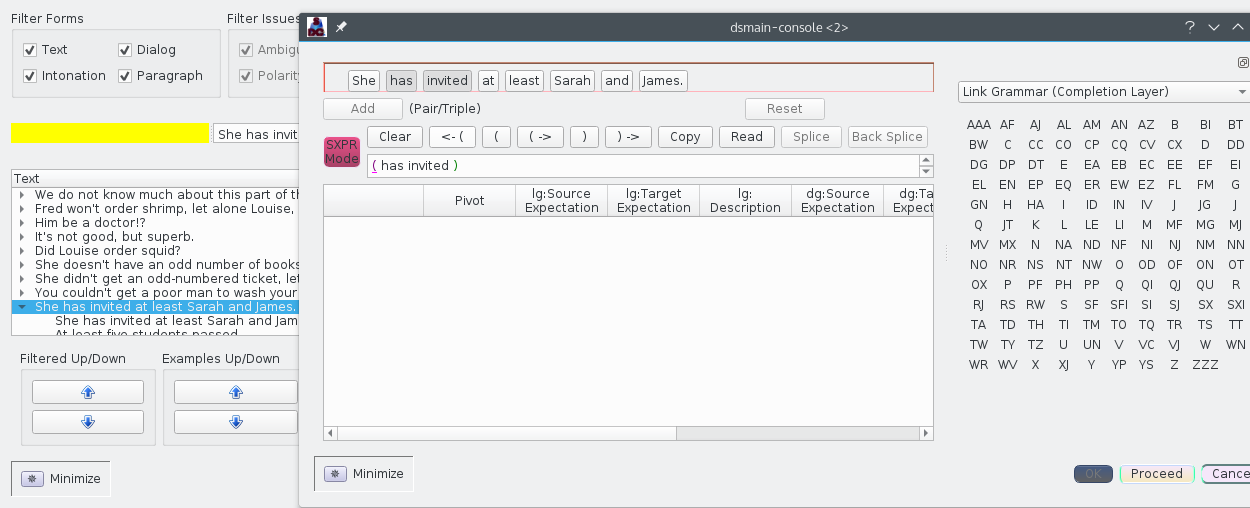
\includegraphics[trim={3.cm 0 0 0},clip]{texs/sxpr.png}}  
        	
      \node [text width=8cm,inner sep=14pt,align=justify,fill=logoCyan!20, draw=logoBlue, 
      draw opacity=0.5,line width=1mm, fill opacity=0.9]
      at (0.41,0.36){\annfont\textbf{The main Dataset Application 
      		for the demo Linguistics data set includes a 
      		distinct window for building annotations on language examples. 
      		Features of this component include an entry area 
      		for building S-Expression models of sentences with visual cues 
      		such as parenthesis-matching color highlights (\circled{1})
      		and sidebars where users can add inter-word annotations using 
      		relations drawn from Link Grammar and 
      		CoNLL-U Dependency Grammar (\circled{2}).}};
          	
 \annotatedFigureBox{0.221,0.655}{0.323,0.696}{1}{0.323,0.696}%
 
 \annotatedFigureBox{0.74,0.27}{0.9985,0.85}{2}{0.76,0.85}%
 
        \end{annotatedFigure}


\end{frame}

